%
% Verification Of Cloud Quantum Computing
%

\section{Verification of cloud quantum computing} \index{Verification}\label{sec:verification}

\subsection{Randomised benchmarking}\label{sec:rand_bench}\index{Randomised benchmarking}

\comment{Insert}

\subsection{Zero-knowledge proofs}\label{sec:ZKP}\index{Zero-knowledge proofs}

Works for all \textbf{NP}-complete problems.

Alg.~\ref{alg:ZKP_graph}

Fig.~\ref{fig:ZKP_graph}

\begin{figure*}[!htpb]
	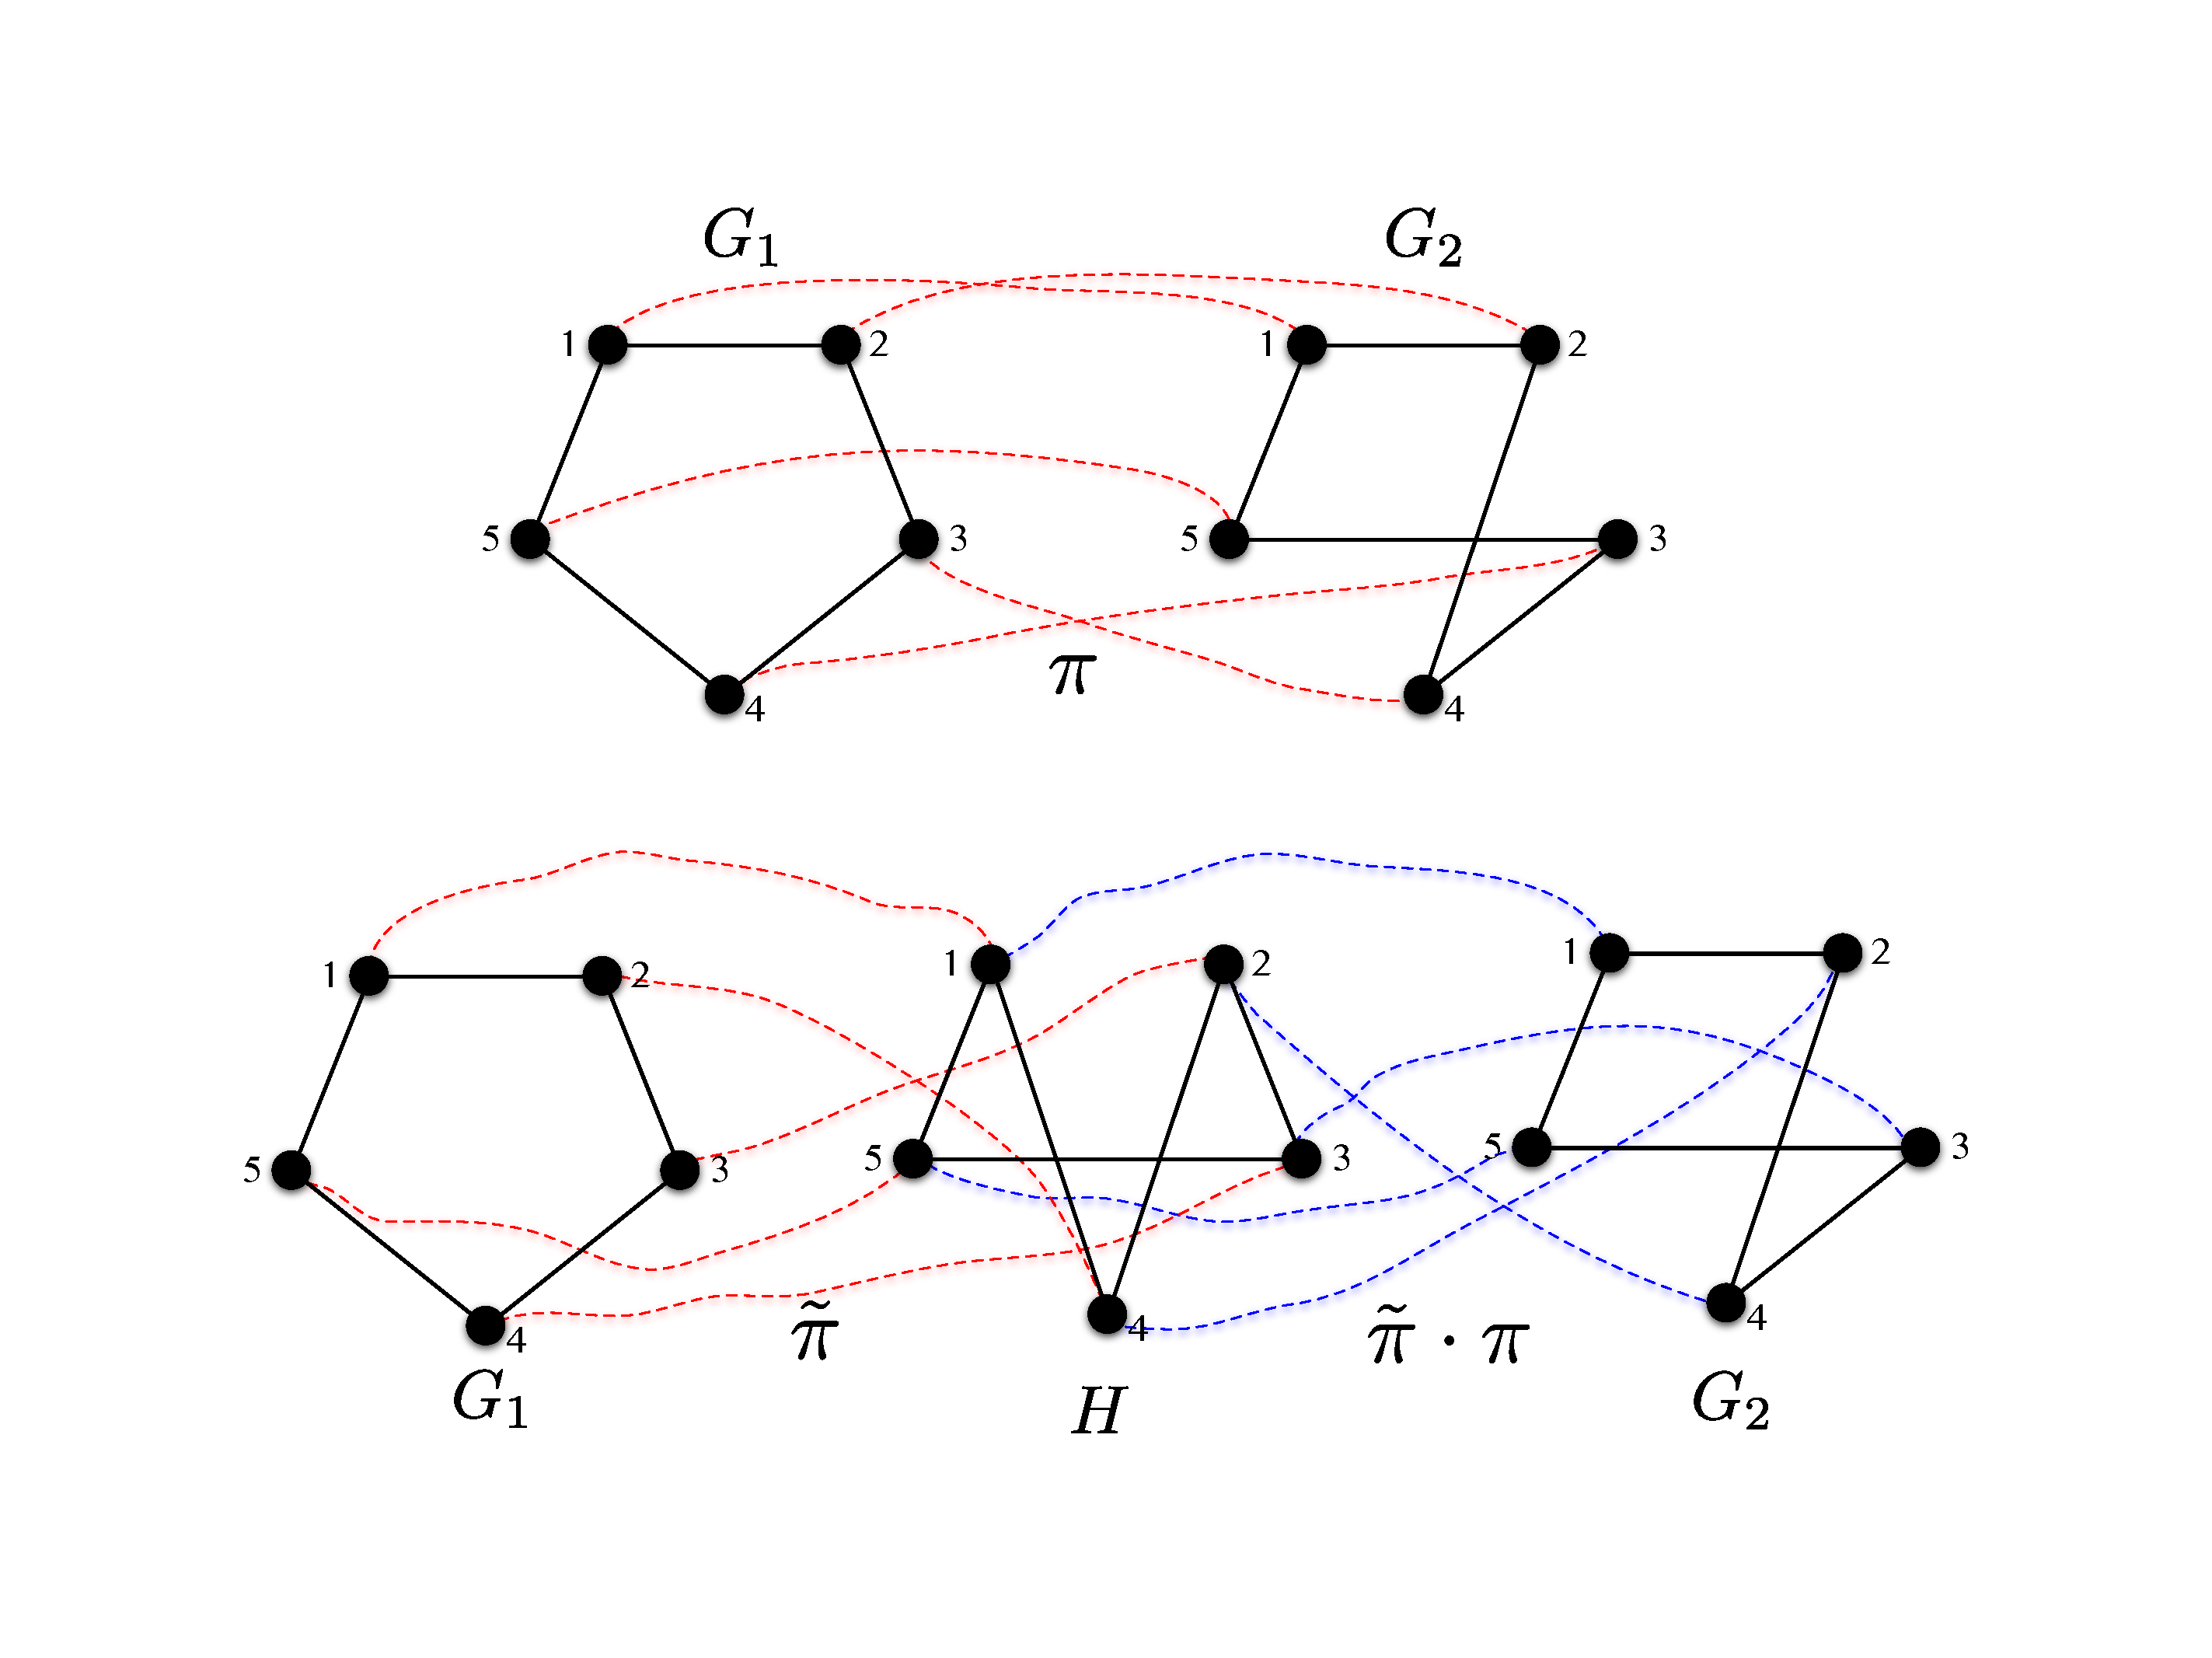
\includegraphics[clip=true, width=\textwidth]{ZKP_graph_isomorphism}
\captionspacefig \caption{\comment{to do}}\label{fig:ZKP_graph}
\end{figure*}

\begin{table}[!htbp]
\begin{mdframed}[innertopmargin=3pt, innerbottommargin=3pt, nobreak]
\texttt{
function ZKP.GraphIsomorphism($G_1$, $G_2$):
\begin{enumerate}
	\item Graphs $G_1$ and $G_2$ are known to both verifier Victor, and prover Peggy.
	\item Peggy knows the permutation $\pi$ for the isomorphism \mbox{$G_1\sim G_2$},
	\begin{align}
		G_1 = \pi \cdot G_2.
	\end{align}
	\item Peggy wishes to prove to Victor that she knows $\pi$, without disclosing what it is.
	\item Peggy chooses another random permutation $\tilde\pi$, and constructs the new permuted matrix $H$,
	\begin{align}
		H &= {\tilde\pi}\cdot G_1,\nonumber\\
		H &= {\tilde\pi}\cdot \pi \cdot G_2.
	\end{align}
	\item Peggy shares $H$ with Victor, randomly isomorphic to both $G_1$ and $G_2$.
	\item Victor randomly (\mbox{$p=1/2$}) asks Peggy to prove \textit{either} \mbox{$H\sim G_1$} \mbox{$H\sim G_2$}.
	\item She reveals either $\tilde\pi$ or \mbox{$\tilde\pi\cdot\pi$} to Victor. He can now efficiently verify either \mbox{$H\sim G_1$} or \mbox{$H\sim G_2$} respectively, by performing the inverse permutation,
	\begin{align}
		G_1 &= {\tilde\pi}^{-1} \cdot H,\nonumber\\
		G_2 &= ({\tilde\pi}\cdot \pi)^{-1} \cdot H.
	\end{align}
	\item Victor is unable to determine $\pi$ from either scenario.
	\item The above is repeated $n$ times. Each time, Peggy chooses a new random $\tilde\pi$.
	\item If Peggy does not actually know $\pi$, the probability of fraudulently passing this test is,
	\begin{align}
		P_\text{deceive} = \frac{1}{2^n}	.
	\end{align}
	\item With error probability $P_\text{deceive}$, Victor knows that Peggy knows $\pi$ for \mbox{$G_1\sim G_2$}.
	\item $\Box$
\end{enumerate}}
\end{mdframed}
\captionspacealg \caption{A zero-knowledge proof for the graph isomorphism problem, an \textbf{NP}-complete problem. Victor (verifier) provides two graphs, $G_1$ and $G_2$, to Peggy (prover), who can demonstrate with asymptotic certainty that she knows the isomorphism \mbox{$G_1\sim G_2$}, without disclosing the permutation $\pi$ that relates them.} \label{alg:ZKP_graph}\index{Zero-knowledge proofs}\index{Graph isomorphism}
\end{table}

\comment{Insert}